\documentclass[a4paper,12pt]{article}

\usepackage{amsmath,amssymb,amsthm,tikz}
\usetikzlibrary{calc,arrows.meta}
\usepackage[margin=20mm]{geometry}


\setlength{\parindent}{0pt}
%\setlength{\columnsep}{1cm}


\begin{document}

%\twocolumn

\thispagestyle{empty}

\begin{center}
{\Large Assignment 4. 2020-10-07},\\
{\em 12 minutes} 
\end{center}

\noindent


{\bf Question 1 (Pointer structure).} Given the starting state 
(shown in the image) and the pseudocode, draw 2 pictures 
showing the pointer states after Line 7 and Line 12 of the code.
In this example $a,b,c$ are the last three digits of your Student ID.

\vspace{10pt}
\begin{tabular}[t]{@{}ll@{}} 
\begin{minipage}[t]{0.68\columnwidth}
Initial state of the pointers/nodes:
\begin{center}
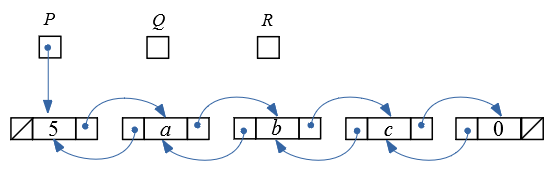
\includegraphics[width=4in]{assignment04-pointers/assignment4-nodes.png}
\end{center}

\end{minipage} &
\begin{minipage}[t]{0.25\columnwidth}

The structure of a single node:

\begin{center}
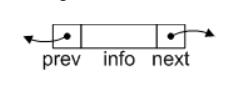
\includegraphics[width=1.5in]{assignment04-pointers/sample-assignment04-structure.png}
\end{center}


\end{minipage}
\end{tabular}


\[
\begin{array}{rl}
1 & Q = P\\
2 & Q = Q\rightarrow next\\
3 & R = Q\rightarrow next\\
4 & \text{\textbf{if\ }} Q\rightarrow info \leq P\rightarrow info\\
5 & \hspace{.5cm} R\rightarrow prev = P\\
6 & \text{\textbf{else\ }}\\
7 & \hspace{.5cm} P\rightarrow  prev = R\\
  & \text{\em (Picture\ 1:\ Show\ the\ pointers\ at\ this\ point) }\\
8 & P\rightarrow next\rightarrow next = R\rightarrow next\\
9 & \text{\textbf{if\ }} R\rightarrow info \leq Q\rightarrow info\\
10 & \hspace{.5cm} R\rightarrow next = P\rightarrow next\\
11 & \text{\textbf{else\ }}\\
12 & \hspace{.5cm} R\rightarrow next = P\rightarrow prev\\
  & \text{\em (Picture\ 2:\ Show\ the\ pointers\ at\ this\ point) }\\

\end{array}
\]




\end{document}



